\newpage
\section{Test 1}
\label{Sec:test_1}

This test is divided into two sub-cases.

\subsection{Normal restitution coefficient set to $\boldsymbol{eps_{n} = 0.0}$}

In the first test setting rover falls freely from the height of 2 meters onto a horizontal plane.
No torques are applied in any of the joints. The only external forces acting on the rover are
the gravity and the ground reaction forces. Initial position of the rover has been set to (x, y, z) = (5, 5, 2) [m].
Friction coefficient has been set to 0.7. In this sub-case restitution coefficients (tangential and normal) have been set to zero. 

\begin{figure}[H]
  \centering
    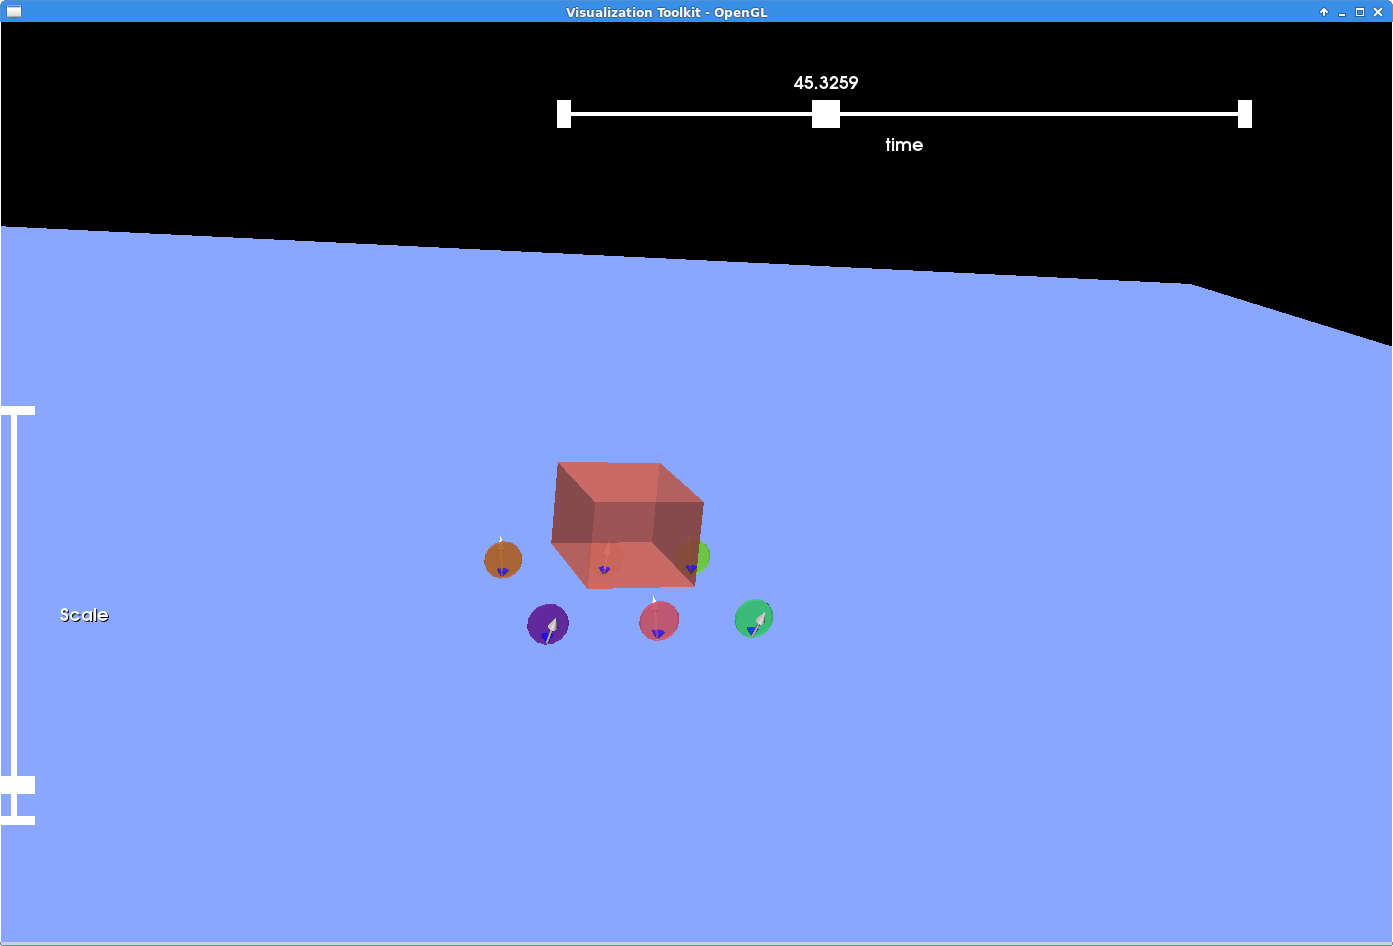
\includegraphics[width=0.8\textwidth]{run_1}
  \caption{First test setting (arrows depict contact forces)}
\end{figure}

\noindent The following essential quantities have been plotted in this case:

\begin{figure}[H]
  \centering
    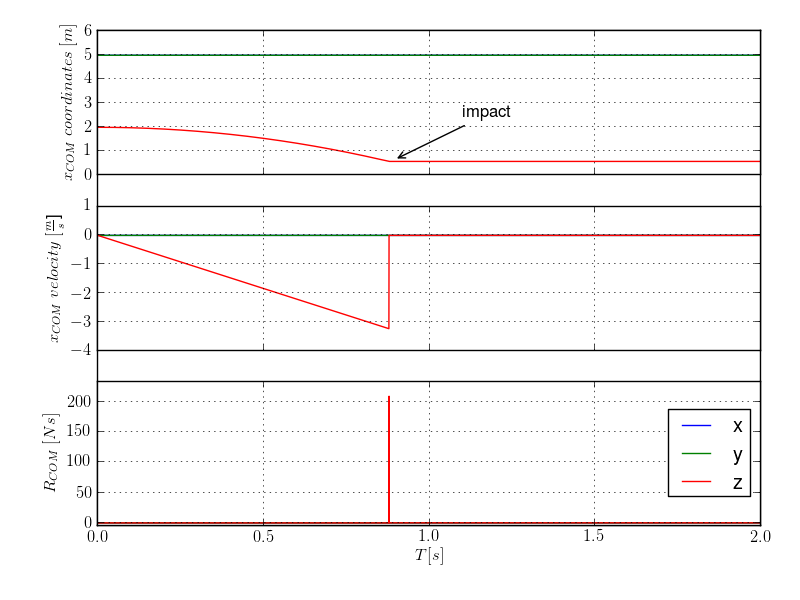
\includegraphics[width=0.8\textwidth]{xvpCOM}
  \caption{Position, velocity and reaction forces of the center of mass}
\end{figure}

\noindent \textbf{\textit{\Large{Comments}}}\\[1mm]
\noindent As seen in the figure 4, coordinate z of the center of mass of the rover decreases parabolically until the system is stable on the plane. This represents the
free-fall phase under gravity. After reaching the plane there is no rebound as the coefficient of restitution in the nonsmooth contact law has been set to zero. Impact corresponds to a 
sharp peak in the force as seen in the third sub-figure.

\noindent Also, the following complimentary quantities have been plotted:

\begin{figure}[H]
  \centering
    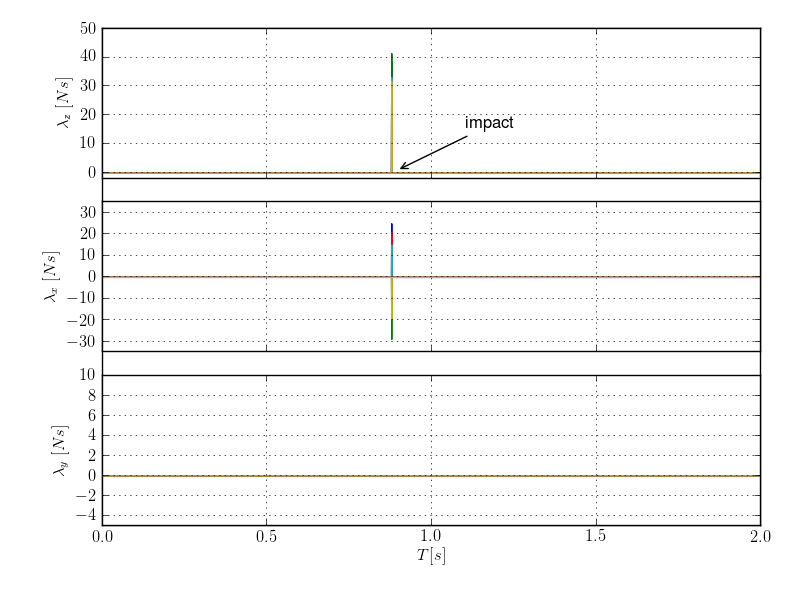
\includegraphics[width=0.8\textwidth]{lambdaNTS}
  \caption{Normal and tangential components of the local contact force (impulsion $\lambda$) for each wheel during impact}
\end{figure}

\begin{figure}[H]
  \centering
    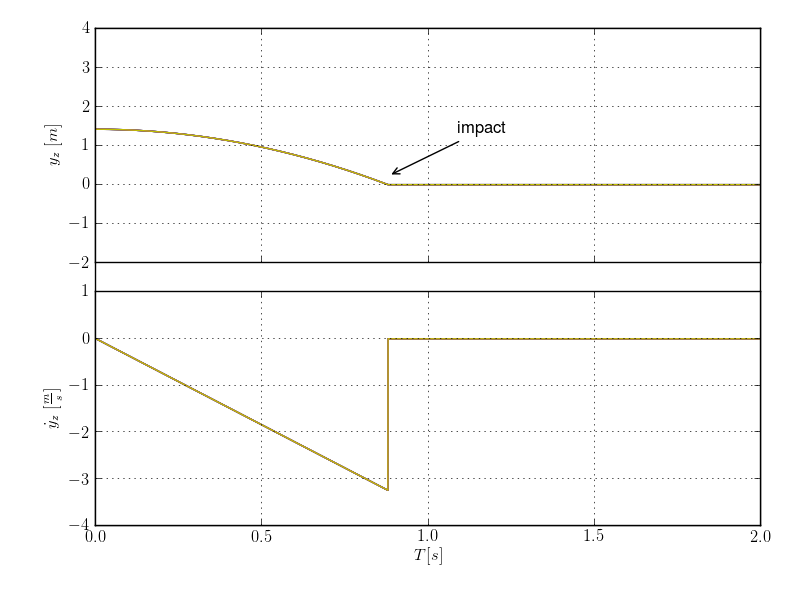
\includegraphics[width=0.8\textwidth]{yNyNdot}
  \caption{$y_{N}$ - gap function (distance between contact point and the constraint function) for each wheel and $\dot{y}_{N}$ - normal component of the local contact velocity for each wheel}
\end{figure}

\noindent \textbf{\textit{\Large{Comments}}}\\[1mm]
\noindent Plots in the figure 5 correspond to forces (normal and tangential impulsions) computed in the local contact frame.
Contact forces are always computed in the local frame and then expressed in the coordinates of the system using jacobian matrix of the constraint function. 
Constraint function (gap function) used to detect the contact and the relative velocity are plotted in the figures 6. Gap function is a relative distance between two contacting
bodies and it imposes geometric constraints on the system. Once slightly below zero it will trigger a nonsmooth interaction between those bodies.\\ 

\subsection{Normal restitution coefficient set to $\boldsymbol{eps_{n} = 0.2}$}

\begin{figure}[H]
  \centering
    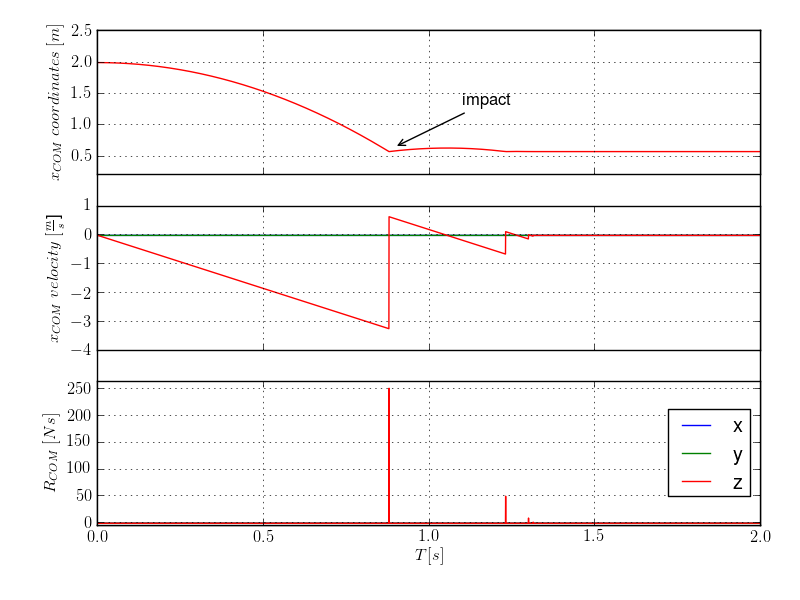
\includegraphics[width=0.8\textwidth]{xvpCOMrest}
  \caption{Position, velocity and reaction forces of the center of mass}
\end{figure}

\noindent \textbf{\textit{\Large{Comments}}}\\[1mm]
\noindent As the restitution coefficient has been set to a non-zero value in this case one observes multiple impacts. Impacts corresponds to peaks of forces in the third sub-figure and 
nonsmooth changes of velocity in the second sub-figure. As the energy is dissipated the magnitudes of impacts reduce in time.\\

\noindent Also, the following complimentary quantities have been plotted:

\begin{figure}[H]
  \centering
    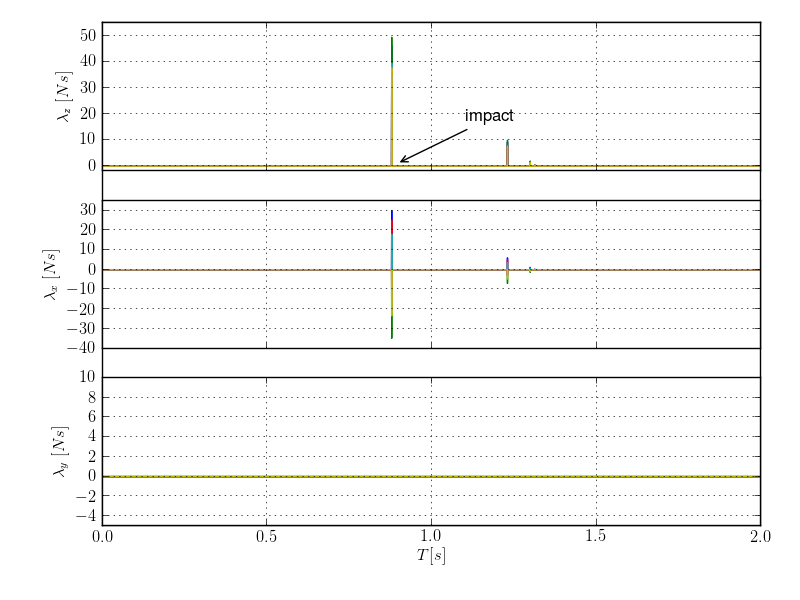
\includegraphics[width=0.8\textwidth]{lambdaNTSrest}
  \caption{Normal and tangential components of the local contact force (impulsion $\lambda$) for each wheel during impact}
\end{figure}

\begin{figure}[H]
  \centering
    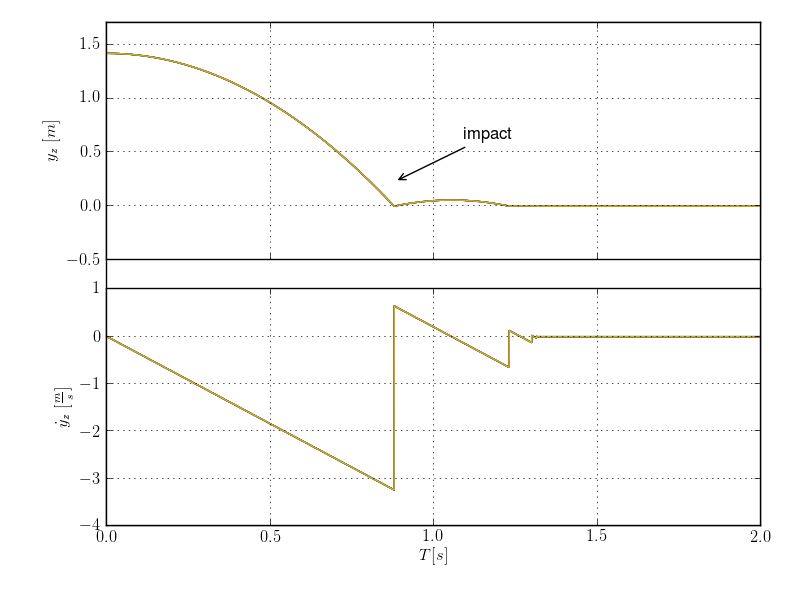
\includegraphics[width=0.8\textwidth]{yNyNdotrest}
  \caption{$y_{N}$ - gap function (distance between contact point and the constraint function) for each wheel and $\dot{y}_{N}$ - normal component of the local contact velocity for each wheel}
\end{figure}

\noindent \textbf{\textit{\Large{Comments}}}\\[1mm]
\noindent In the figure 9 one can see the gap function and relative velocity plots. With respect to the previous sub-case rebounds off the ground are visible.\\ 

